% - Why is asset allocation important? Short description of the asset allocation optimisation problem.
% - Short history of Markowitz's Modern Portfolio Theory.

In this section, we provide a general definition of the asset allocation problem, and define two naive solutions as well as Markowitz's solution to this problem. Finally, we present the results of simulating these three allocation methods during the year 2020.

Assume an investor with a total wealth of $\$x \in \mathbb{R}_{\geq 0}$, i.e. a total wealth of $x$ U.S. dollars. Let $A := \{a_1, \dots, a_N \}$ be the set of assets, which the investor can trade (buy and sell) and let $a_i$ be the real-valued random variable representing the return of asset $i = \{ 1, \dots, N \}$. By asset, we understand anything with a price that can be bought and sold so as to profit from price differences across time and that might also produce some cash-flow (coupon or dividend payments), i.e. returns. However, here we will focus on the most widely used investment assets: for example cash, real-estate objects, bonds, stocks, commodities and funds.

\begin{definition}
    A \textbf{portfolio $P_A$ composed of the assets in $A$} is defined as
    \begin{align*}
        P_A = \begin{bmatrix} w_1 \\ \vdots \\ w_N \end{bmatrix} \in \mathbb{R}^N, \quad \text{such that} \quad \sum_{i=1}^N w_i = 1,
    \end{align*}
    where each weight $w_i$ represents the relative allocation of the investor's total wealth to asset $i = \{ 1, \dots, N \}$. The real-valued random variable $X$ which represents the returns of the portfolio $P_A$ is given by
    \begin{align*}
        X = \sum_{i=1}^N w_i a_i.
    \end{align*}
\end{definition}

One of the most important questions that an investor faces is how much of their total wealth $\$x$ they should allocate to each of the assets in $A$, i.e. which portfolio $P_A \in \mathbb{R}^N$ they should to hold. This question has infinite discretionary and many systematic answers. For example, wealthy investors might prefer to hold a portfolio focused on protecting their total wealth against inflation and other risks, while less affluent investors might prefer a portfolio with a high growth potential at the expense of assuming higher risks.

\subsection{Naive Portfolio Allocation Models}
    One of the most naive answers to this question is to allocate an equal amount of wealth to each asset. Another naive answer is to allocate wealth to each asset according to their returns' variance, so that each asset is allocated in inverse proportion to their returns' variance.
    
    \begin{definition}[Equal Weight Portfolio \cite{equalweight}]\label{definition:EqualWeightPortfolio}
        Consider the set of investable assets $A = \{ a_1, \dots, a_N \}$. The \textbf{equal weight allocation portfolio (EWP)} is defined as
        \begin{align*}
            EWP_A = [w_i] \in \mathbb{R}_{\geq 0}^N, \quad \text{such that} \quad w_i := \frac{1}{N} \quad \text{for all} \quad i = 1, \dots, N.
        \end{align*}
    \end{definition}
    
    The equal weight portfolio is the most widely used allocation method when no information about the assets in the portfolio is available to rank them or to compute some measure to define an optimisation problem. It is also the most naive way of allocating capital across the $N$ assets considered. However, this naive method has proven to perform even better than other, even very sophisticated, methods as shown in \cite{equalweight}.
    
    \begin{definition}[Inverse Variance Portfolio \cite{equalweight}]\label{definition:InverseVariancePortfolio}
       Consider the set of investable assets $A = \{ a_1, \dots, a_N \}$. The \textbf{inverse variance allocation portfolio (IVP)} is defined as
        \begin{align*}
            IVP_A = [w_i] \in \mathbb{R}_{\geq 0}^N, \quad \text{such that} \quad w_i := \frac{\frac{1}{\mathbb{V}[a_i]}}{\sum_{k=1}^N \frac{1}{\mathbb{V}[a_k]}} \quad \text{for} \quad i=1, \dots, N,
        \end{align*}
        where $\mathbb{V}[a_i]$ is the variance of the returns' distribution of the $i$-th asset.
    \end{definition}
    
    The IVP can be understood as the allocation method that weights each asset in the portfolio so that each of them contributes the same amount to the total portfolio risk if the returns of assets are considered stochastic independent (assets with higher variance are allocated a smaller portion of the portfolio than assets with lower variance).
    
    Although IVP is more complex than the EWP model because the estimation of some parameters is needed, it is still considered a naive method.

\subsection{Markowitz's Portfolio Optimisation Model}
    Harry M. Markowitz was the first to develop and present a systematic approach to mathematically define superior portfolios, i.e. portfolios that an investor would prefer to hold irrespective of the investors' goals or constrains. Moreover, he gave a mathematical definition for measuring risk by defining it as the standard deviation of past returns and also a mathematical definition for measuring future returns by using the expected value of past returns. His work earned him a Nobel Memorial Prize in Economic Sciences in 1990 \cite{markowitznobelprize}. Markowitz's portfolio construction model laid the ground for quantitative asset allocation models. Many asset allocation models today are developed using Markowitz's model and adjusting it to account for modern investors' needs. For example, by using risk measures other than the standard deviation of past returns, or by targeting functions other than expected returns.
    
    The most important parameter in the optimisation problem that defines the elements in the set of superior portfolios that Markowitz defined is the sample covariance matrix of asset returns.
    
    \begin{definition}[Sample Covariance, Variance, Standard Deviation and Correlation Matrices of Asset Returns]\label{definition:CovarianceMatrix}
       Let $R = [r_{n,t}] \in \mathbb{R}^{N \times T}$ be the matrix that contains $T \in \mathbb{N}$ observations of the $\{ a_1, \dots, a_N \}$ real-valued random variables of asset returns. Moreover, let the matrix of centred returns be defined as
       \begin{align*}
           \tilde{R} = [\tilde{r}_{n,t}] \in \mathbb{R}^{N \times T}, \quad \text{where} \quad \tilde{r}_{n,t} := r_{n,t} - \frac{1}{T} \sum_{i=1}^T r_{n,i}.
       \end{align*}
       Then, the \textbf{$T$-periods sample covariance matrix of asset returns} is defined as
       \begin{align*}
           \Sigma = [\sigma_{i,j}] := \frac{1}{T} \left( \Tilde{R} \Tilde{R}^T \right) \in \mathbb{R}^{N \times N},
       \end{align*}
       where $\sigma_{i,j}$ represents the $T$-periods sample covariance of the $i$-th and $j$-th assets. Finally, we define the \textbf{variance matrix} $V = [v_{i,j}] := diag(\sigma_{i,j}) \in \mathbb{R}^{N \times N}$, the \textbf{standard deviation matrix} $S = [s_{i,j}] := V^{\frac{1}{2}} \in \mathbb{R}^{N \times N}$ and the \textbf{correlation matrix}
       \begin{align*}
           P = [\rho_{i,j}] := S^{-1} \Sigma S^{-1} \in \mathbb{R}^{N \times N}.
       \end{align*}
    \end{definition}
    
    \begin{remark}[\cite{besselcorrection}]\label{remark:UnbiasedSampleCovarianceMatrix}
        Because we do not know the true mean return of each asset and use the sample mean to compute the sample covariance matrix, we need to use Bessel's correction to get an unbiased estimator of the sample covariance matrix. That is an estimator that is equal to its expected value. Let $T > 1$ and $\Sigma, V, S$ be the sample covariance, variance and standard deviation matrices defined above respectively, then their unbiased estimators are given by
        \begin{align*}
            \Sigma_{unbiased} &:= \frac{T}{T-1} \Sigma, \\
            V_{unbiased} &:= \frac{T}{T-1} V, \\
            S_{unbiased} &:= \frac{T}{T-1} S.
        \end{align*}
        From now on, when we refer to the sample covariance, variance and standard deviation matrices, we refer to them after Bessel's correction.
    \end{remark}
    
    %\begin{theorem}\label{theorem:CovarianceMatrixRank}
    %    Let $R, \tilde{R}, \Sigma$ be as in definition \ref{definition:CovarianceMatrix}. If $\Sigma \in GL_N(\mathbb{R})$, then $rank(R) = N$ holds.
    %\end{theorem}
    %
    %\begin{proof}
    %    If $\Sigma \in GL_N(\mathbb{R})$, then
    %    \todo[inline]{Liesen: why $rank(\Tilde{R}) \leq rank(R)$? \url{https://math.stackexchange.com/questions/3721486/how-is-the-rank-of-a-matrix-affected-by-centering-the-columns-of-a-matrix/3721511} \url{https://en.wikipedia.org/wiki/Centering_matrix}}
    %    \begin{align*}
    %        N = rank(\Sigma) \leq rank \left( \frac{1}{T} \left( \Tilde{R} \Tilde{R}^T \right) \right) \leq rank(\Tilde{R}).% \leq rank(R) \leq \min \{ N, T \}
    %    \end{align*}
    %    
    %    Moreover, can rewrite the matrix of centered returns as $\Tilde{R} = R (I_N - \frac{1}{T} \mathds{1} \mathds{1}^T)$.
    %    
    %    Hence, $rank(R) = N$ and $N \leq T$ must hold.
    %\end{proof}
    %
    %\begin{remark}
    %    Theorem \ref{theorem:CovarianceMatrixRank} also applies to the unbiased sample covariance matrix from remark \ref{remark:UnbiasedSampleCovarianceMatrix}, because the unbiased sample covariance matrix differs from the biased sample covariance matrix from \ref{definition:CovarianceMatrix} only by a non-zero scalar factor.
    %\end{remark}
    
    Now that we have defined the sample covariance matrix of asset returns, we can proceed to define the elements of the set of superior portfolios.
    
    \begin{definition}[Optimal Mean-Variance Portfolio \cite{markowitzorg}]\label{definition:OptimalMeanVariancePortfolio}
        Consider the set of investable assets $A = \{ a_1, \dots, a_N \}$. Then \textbf{Markowitz's optimal portfolio for a given level of return $\mu_P \in \mathbb{R}$} is given by the solution to the optimisation problem
        \begin{align*}
            \arg \min_{w \in \mathbb{R}^N}& \quad w^T \Sigma w, \\
            \text{s.t.}& \quad \mathds{1}^T w = 1, \\
            & \quad \mu^T w = \mu_P,
        \end{align*}
        where $\mathds{1} := [ 1, \dots, 1]^T \in \mathbb{R}^N$, $\Sigma \in \mathbb{R}^{N \times N}$ is the sample covariance matrix of returns and $\mu \in \mathbb{R}^N$ is the vector of expected returns of the $N$ assets.
        
        The set of pairs $(\mu_p, \sigma_P^2) \in \mathbb{R} \times \mathbb{R}_{\geq 0}$ such that, for each $\mu_P \in \mathbb{R}$, $\sigma_P^2 := w_{opt}^T \Sigma w_{opt}$, where $w_{opt}$ is the solution to the optimisation problem above, is called the \textbf{efficient frontier}.
    \end{definition}
    
    Please, note that, while the equal weight and inverse variance portfolios are long-only portfolios (all assets are either bought or not bought), Markowitz's optimal portfolios are long-short portfolios, i.e. short-selling\footnote{Short-selling is the act of selling an asset that you do not own by borrowing it and later re-buying it to hand it back to the borrower, so as to profit from the fall in the price of the asset.} is allowed. Mathematically, this means that the optimal vector solution to the optimisation problem in definition \ref{definition:OptimalMeanVariancePortfolio} can contain negative entries, while the equal weight and inverse variance portfolio vectors only contain non-negative entries. Obviously, zero entries are can appear in all three of them, meaning that the corresponding asset is not part of the portfolio.
    
    An investor that wants to select an optimal portfolio using Markowitz's model can then decide to either
    \begin{enumerate}
        \item choose a portfolio in the efficient frontier by specifying a target level of portfolio return $\mu_P$ (this corresponds to selecting the portfolio with the specified target expected return with the minimum variance of returns),
        \item or choose a portfolio in the efficient frontier by specifying a target level of risk $\sigma_P^2$ (this corresponds to selecting the portfolio with the specified level of returns' variance with the maximum expected return).
    \end{enumerate}
    
    Because most investors do not have very precise target return or target risk level for their portfolios, Markowitz applied the concept of utility function maximisation to the process of portfolio selection. Utility functions can have many forms, but Markowitz defined them as functions of the form
    \begin{align}\label{equation:UtilityFunction}
        U_{\alpha}(w_P) := \mu_P - \frac{1}{2 \alpha} \sigma_P^2 = w_P^T \mu  - \frac{1}{2 \alpha} w_P^T \Sigma w_P, \quad \alpha \neq 0,
    \end{align}
    using the notation from definition \ref{definition:OptimalMeanVariancePortfolio}.
    
    This utility function is a measure of investor happiness. The more risk averse the investor, the less happy the investor will be with high variance of portfolio returns and hence the nearer the value of $\alpha$ will be to $0$. Each investor has his/her own utility function, and this utility function can also change over time as the financial situation of the investor changes. Markowitz assumes that all investors are risk-averse. For risk-seeking investors, i.e. investors that prefer portfolios with higher variance for a fixed given level of target return, the factor $\alpha$ would be negative. However, we will ignore risk-seeking ($\alpha < 0$) and risk-indifferent ($\alpha = 0$) investors here.
    
    Markowitz argues that an investor should choose the portfolio that maximises his/her utility function. We can compute such a portfolio by taking the derivative of the general utility function defined in equation \ref{equation:UtilityFunction} and setting it to zero, because the utility function is convex for all $\alpha > 0$. The optimal portfolio is then given by the solution to the linear system
    \begin{align*}
        \frac{\partial U_{\alpha}}{\partial w_P} = \mu - \frac{1}{\alpha} \Sigma w_P = 0 \Leftrightarrow \Sigma w_P = \alpha \mu.
    \end{align*}
    
    It is important to mention that the portfolio corresponding to the solution of the linear system above might not add up to $1$, and we can understand the parameter $\alpha$ as a factor for the optimal leverage , i.e. if the investor should borrow money to invest in the portfolio $P$ on top of his/her total wealth ($\sum_{i=1}^N w_{Pi} > 1$), invest all its wealth without borrowing ($\sum_{i=1}^N w_{Pi} = 1$) or only invest a part of its total wealth in the portfolio $P$ ($\sum_{i=1}^N w_{Pi} < 1$).
    
    \begin{example}
        Consider a set of investable assets $A = \{ a_1, a_2 \}$, such that their expected returns' vector is given by $\mu = \begin{bmatrix} 1 \\ 1 \end{bmatrix}$ and the covariance matrix of returns by $\Sigma = I_2$. Then the utility maximising portfolio is equal to $w_P = \alpha \mu$.
        
        Investors with an utility function $U_{\alpha}$, $\alpha \in (0, 0.5)$ would only invest a portion ($2 \alpha$) of their total wealth in the portfolio. Investors with an utility function $U_{\alpha}$, $\alpha = 0.5$ would invest their complete wealth in the portfolio. Finally, investors with an utility function $U_{\alpha}$, $\alpha > 0.5$ would not only invest their complete wealth, but also borrow extra wealth to also invest it in the portfolio.
    \end{example}
    
    A common misconception when talking about Markowitz's optimal portfolios is that their computation assumes that returns are normally distributed. This is however wrong, as we have not used this assumption yet, and will not use it later. However, it is true that Markowitz's optimal portfolios are utility maximising only if the utility function of the investor is dependent on first and second order movements of returns, i.e. dependent on mean return and variance of returns. For investors, whose utility function also depends on variables other than portfolio mean return and variance of returns, Markowitz's optimal portfolios might not be optimal. For example, if the investor's utility is also dependent on the maximum temporal loss or the skewness of returns.
    
    The main critique point of this optimisation problem is the high sensitivity to small changes in the expected returns vector $\mu$, which, as mentioned before, is defined as the vector of sample mean of the past $T$-periods asset returns. This leads to significantly different portfolio allocations even with an unchanged sample covariance matrix as argued in -\cite{michaudreturnsstability}, which in turn leads to a high portfolio turn-over and to concentrated portfolios, especially when correlations rise. Because returns are difficult to forecast accurately enough to keep the sensitivity within certain limits, some asset managers abstain from using them as input parameter. Portfolio allocations are then computed on the basis of the sample covariance matrix only, which is a risk parameter, hence the name \textit{risk-based} asset allocation. In the case of Markowitz's portfolio optimisation model, risk-based optimal portfolios correspond to minimum volatility portfolios.
    
    \begin{definition}[Minimum Volatility Portfolio \cite{berndscherer}]\label{definition:MinimumVolatilityPortfolio}
        Consider the set of investable assets $A = \{ a_1, \dots, a_N \}$. Then the \textbf{minimum volatility portfolio}\footnote{Markowitz defines volatility as the standard deviation of returns. Therefore, the minimum volatility portfolio is also the minimum variance portfolio.} is given by the solution to the optimisation problem
        \begin{align*}
            \arg \min_{w \in \mathbb{R}^N}& \quad w^T \Sigma w, \\
            \text{s.t.}& \quad \mathds{1}^T w = 1.
        \end{align*}
    	The minimum volatility portfolio is also a long-short portfolio, i.e. the portfolio might contain negative weights for some assets.
    \end{definition}
    
    %\begin{remark}
    %    The minimum volatility portfolio optimisation problem is equivalent to the following
    %    \begin{align*}
    %        \arg \min_{w \in \mathbb{R}^N}& \quad \frac{1}{2} w^T \Sigma w \\
    %        \text{s.t.}& \quad \mathds{1}^T w = 1
    %    \end{align*}
    %\end{remark}
    
    \begin{theorem}
        Assuming that $\Sigma$ is non-singular, the minimum volatility portfolio allocation vector is given by
        \begin{align*}
            w_{opt} := \frac{1}{\mathds{1}^T \Sigma^{-1} \mathds{1}} \Sigma^{-1} \mathds{1}.
        \end{align*}
    \end{theorem}
    
    \begin{proof}
        We define the Lagrangian corresponding to the minimum volatility portfolio optimisation problem as
        \begin{align*}
            \mathcal{L}(w, \lambda) := w^T \Sigma w - \lambda (\mathds{1}^T w - 1).
        \end{align*}
        
        Because a non-singular sample covariance matrix is positive-definite and we have a quadratic optimisation problem, we only need to take the first derivatives with respect to both $w$ and $\lambda$, and set them to zero to find the solution of the optimisation problem, i.e.,
        \begin{align*}
            0 = 2 \Sigma w - \lambda \mathds{1} &\Leftrightarrow w = \frac{\lambda}{2} \Sigma^{-1} \mathds{1}, \\
            \text{and } 0 = 1 - \mathds{1}^T w &\Leftrightarrow \lambda = \frac{2}{\mathds{1}^T \Sigma^{-1} \mathds{1}}.
        \end{align*}
        Hence,
        \begin{align*}
            w_{opt} := \frac{\frac{2}{\mathds{1}^T \Sigma^{-1} \mathds{1}}}{2} \Sigma^{-1} \mathds{1} = \frac{1}{\mathds{1}^T \Sigma^{-1} \mathds{1}} \Sigma^{-1} \mathds{1}.
        \end{align*}
    \end{proof}
    
    The analytical expression for $w_{opt}$ presented above contains the inverse of the sample covariance matrix. Because covariance matrices are only positive-semidefinite, i.e. not necessarily non-singular, and because computing the inverse of a matrix is computationally very expensive, we prefer to define $w_{opt}$ as the solution for a linear system.
    
    \begin{algorithm}[H]\label{algorithm:MMVP}
        \SetAlgoLined
        \SetKwInOut{Input}{Input}\SetKwInOut{Output}{Output}
        \Input{$N$-Asset return matrix $R \in \mathbb{R}^{N \times T}$}
        \Output{Markowitz Minimum Variance Portfolio $w_{opt}$}
        Compute the sample covariance matrix $\Sigma \in \mathbb{R}^{N \times N}$\;
        \If{$\Sigma$ is non-singular}{
        Set $\Tilde{w}_{opt} \in \mathbb{R}^N$ to the solution to $\Sigma w = \mathds{1}$\;}
        \Else{Set $\Tilde{w}_{opt} \in \mathbb{R}^N$\ to one of the solutions to the least-squares problem $\Sigma w = \mathds{1}$\;}
        Set $w_{opt} = \frac{1}{\mathds{1}^T \Tilde{w}_{opt}} \Tilde{w}_{opt}$\;
        \caption{Markowitz Minimum Variance Portfolio Computation}
    \end{algorithm}
    ~\
    
    Note that if $\Sigma$ is singular, we can use the least-squares method to get an optimal portfolio. However, in that case, only $\| \Sigma w_{opt} - \mathds{1} \| = \min_{w \in \mathbb{R}^N} \| \Sigma w - \mathds{1} \|$ holds, and $\Tilde{w}_{opt}$ might not be unique. From now on, we assume that the sample covariance matrix at step 1 has full rank, and is therefore invertible.
    
    \begin{remark}\label{remark:IVPEquivalentToMMVP}
        For the especial case of a covariance matrix that is invertible and diagonal, i.e. if all assets are uncorrelated and with return variances strictly greater than zero, the inverse variance allocation portfolio is equivalent to the Markowitz minimum variance portfolio. This is because in such case, we would only need to solve $N$ linear equations at step 3 of the algorithm \ref{algorithm:MMVP} of the form
        \begin{align*}
            \sigma_{i,i} w_i = 1 \quad \text{for} \quad i = \{ 1, \dots, N \},
        \end{align*}
        where $\sigma_{i,i} = \mathbb{V}[a_i] \in \mathbb{R}_{>0}$ is the returns' variance of the $i$-th asset which lies in the diagonal of $\Sigma$.
        
        Finally, at step 8, we get that
        \begin{align*}
            w_{opt} = \frac{1}{\sum_{k=1}^N \frac{1}{\sigma_{k,k}}} \begin{bmatrix} 
                                                    \frac{1}{\sigma_{1,1}} \\
                                                    \vdots \\
                                                    \frac{1}{\sigma_{N,N}}
                                                \end{bmatrix} = \frac{1}{\sum_{k=1}^N \frac{1}{\mathbb{V}[a_k]}}                     \begin{bmatrix} 
                                                                        \frac{1}{\mathbb{V}[a_1]} \\
                                                                        \vdots \\
                                                                        \frac{1}{\mathbb{V}[a_N]}
                                                                    \end{bmatrix} = IVP_A.
            %[w_i] \in \mathbb{R}_{\geq 0}^N, \quad \text{such that} \quad w_i := \frac{\frac{1}{\mathbb{V}[a_i]}}{\sum_{k=1}^N \frac{1}{\mathbb{V}[a_k]}} \quad \text{for} \quad i=1, \dots, N,
        \end{align*}
        %the solution to the optimisation problem
        %\begin{align*}
        %    \arg \min_{w \in \mathbb{R}^N}& \quad w^T \Sigma w, \\
        %    \text{s.t.}& \quad \mathds{1}^T w = 1,
        %\end{align*}
        %where $\Sigma := diag( \mathbb{V}[a_1], \dots, \mathbb{V}[a_N] )$ such that $a_i$ is the returns distribution of the $i$-th asset. This means that the inverse variance portfolio is the minimum volatility portfolio, that present later, considering all assets uncorrelated.
    \end{remark}
    
    %References: \cite{markowitzorg}, \cite{berndscherer}
    
    \subsection{Practical Implementation of Naive Portfolio Allocation Methods}\label{section:PracticalImplementationofNaivePortfolioAllocationMethods}
        In this subsection, we present the results of the practical implementation of the naive portfolio allocation methods described in definitions \ref{definition:EqualWeightPortfolio} and \ref{definition:InverseVariancePortfolio}, which serve as benchmarks for the Markowitz's minimum volatility portfolios. See appendix \ref{appendix:PracticalImplementationFramework} for details about the selected asset as well as other parameters and tools used to generate the results presented here.
        
        % Tools to analyse PFs: HHI for concentration, risk-adjusted returns, stability: turn-over volume, what else?
        
        The portfolios generated in backtesting by each of the naive optimisation methods and the other methods defined later are compared with respect to risk-adjusted return, concentration and stability. The Sharpe ratio is the chosen measure to quantify risk-adjusted returns. To assess concentration, we will use a normalised version of the Herfindahl-Hirsch-Index (HHI). The normalisation step is necessary, because we will allow for short positions in our portfolios, and the HHI is only defined for positive portfolio weights. We will measure stability via the turnover of the portfolio.
        
        \begin{definition}[Sharpe Ratio \cite{franzen}] % Page 216
            Let $\mu_P \in \mathbb{R}$ be the return of the portfolio $P$ over a given period of time and $\sigma_P \in \mathbb{R}_{\geq 0}$ its standard deviation over that same period of time. Moreover, let $R_f \in \mathbb{R}$ be the risk-free rate of that given period. Then the \textbf{Sharpe Ratio of portfolio $P$ over the given period} $SR_P \in \mathbb{R}$ is given by
            \begin{align*}
                SR_P := \frac{\mu_P - R_f}{\sigma_P}.
            \end{align*}
            
            The risk-free rate is the return of the safest asset available, usually cash deposits at a commercial or central bank or the return of some high-quality short-term government bond like the U.S. treasury bill (\textit{T-Bill}) or the German Federal Treasury notes (\textit{Schatz}).
        \end{definition}
        
        \begin{remark}
            We do not compute the Sharpe ratio of the backtest separately, and rely upon QuantConnect's internal overall portfolio statistics for its computation, i.e. all Sharpe ratios presented here are the Sharpe ratios that appear in QuantConnect's backtesting results. QuantConnect computes the Sharpe ratio using the same definition as above, but using the annualised return of the portfolio in the backtest and assuming a risk-free rate of $0\%$ \cite{qcsharperatiocode}.
        \end{remark}
        
        % https://quant.stackexchange.com/questions/65525/herfindahl-hirsch-index-for-fx-portfolios?noredirect=1#comment92677_65525
        %To assess concentration, we choose Yager's entropy, because, in contrast to the Herfindahl-Hirsch-Index, Yager's entropy allows asset weights to be negative. 
        
        %\begin{definition}[Yager's Entropy \cite{yagerentropy}]
        %    Consider a portfolio with $n$ assets. Let $w_1, \dots, w_n \in \mathbb{R}$ be the weights associated to each of the $n$ assets in the portfolio. Then Yager's entropy $Q(w_1, \dots, w_n)$ is defined as
        %    \begin{align*}
        %        Q(w_1, \dots, w_n) := - \left( \sum_{i=1}^n \left| w_i - \frac{1}{n} \right|^z \right)^{\frac{1}{z}}
        %    \end{align*}
        %    where $z \in \mathbb{N}_{\geq 1}$ is a constant. \todo{change source to \url{https://www.sciencedirect.com/science/article/abs/pii/002002559400030F}}
        %\end{definition}
        
        %\begin{remark}
        %    \todo{add remark, that min entropy if equal weighted portfolio}
        %\end{remark}
        
        \begin{definition}[Herfindahl-Hirsch-Index \cite{chammas}] % Page 71 (85 of the PDF)
            Let $P = [w_i] \in \mathbb{R}_{\geq 0}^N$ be a portfolio, such that $\sum_{i=1}^N w_i = 1$. We define the \textbf{Herfindahl-Hirsch-Index (HHI)} as
            \begin{align*}
                HHI_P := \| P \|_2^2.
            \end{align*}
            For the general case of a portfolio $P = [w_i] \in \mathbb{R}^N$, we define the \textbf{normalised Herfindahl-Hirsch-Index (nHHI)} as
            \begin{align*}
                nHHI_P := \left( \frac{\| P \|_2}{\| P \|_1} \right)^2. %\sum_{i=1}^N \left( \frac{|w_i|}{\sum_{j=1}^N |w_j|}\right)^2
            \end{align*}
            Obviously, $nHHI_P \leq HHI_P$ for all portfolios $P \in \mathbb{R}^N$.
        \end{definition}
        
        \begin{definition}[Turnover \cite{equalweight}]
            Consider a portfolio $P$ with $N$ assets. Let $w_{j,t+1} \in \mathbb{R}$ be the portfolio weight assigned to asset $i$ at time $t$ by the portfolio optimisation method, and let $w_{j,t^+} \in \mathbb{R}$ be the portfolio weight of asset $i$ before rebalancing at time $t+1$ for $i=1, \dots, N$ and $t=0, \dots, T$. The turnover of the portfolio $P$ is defined as
            \begin{align*}
                TO_P := \frac{1}{T} \sum_{t=0}^T \sum_{i=1}^N \left( \left| w_{i, t+1} - w_{i, t^+} \right| \right),
            \end{align*}
            where $T \in \mathbb{N}$ is the number of rebalancing points of the portfolio.
        \end{definition}
        
        This turnover quantity can be interpreted as the average percentage of wealth traded at each rebalancing point.
        
        Now that we have defined the 3 measures which we will use to compared the portfolios resulting from the different portfolio construction models across the backtesting period, we proceed to present the results of the 2 naive portfolio optimisation models from definitions \ref{definition:EqualWeightPortfolio} and \ref{definition:InverseVariancePortfolio}. The vectors with the optimal portfolios computed using these 2 naive methods can be found in appendices \ref{appendix:EWPortfolios} and \ref{appendix:IVPortfolios}.
        
        In figure \ref{fig:ivp_allocation_plot}, a visual representation of the target allocation of all 20 assets in the IVP over the backtesting period is presented. Most of the portfolio's wealth is allocated to ISTB (iShares Core 1-5 Year USD Bond ETF) and IAGG (iShares Core International Aggregate Bond ETF). The allocation to the first drops at the start of the COVID-19 crisis, while the allocation of the second rises. The allocation to IMTB (iShares 5-10 Year USD Bond ETF) rises after the start of the COVID-19 crisis. For the rest of assets the allocation remains relatively stable over the whole backtesting period. Finally, the high allocation to fixed income ETFs is not surprising, because they tend to show lower variance of returns, while the allocation to equity, including real-estate, and commodity ETPs remains low due to the higher variance of returns that they tend to present.
        
        % Data
        \begin{figure}[h]
            \centering
            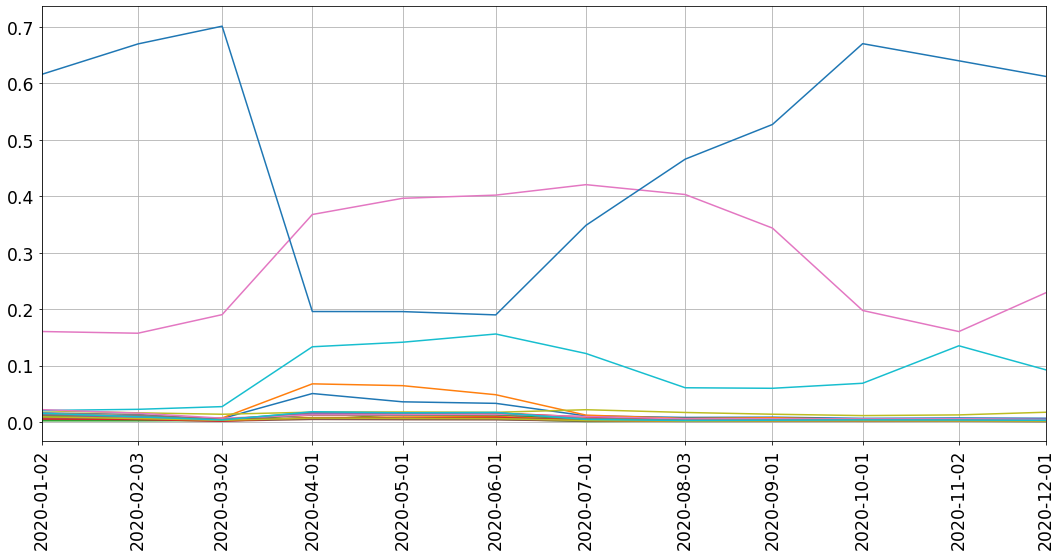
\includegraphics[width=1.15\textwidth]{bilder/IVP_allocation_plot.png}
            \caption{IVP Target Allocation over Time}
            \label{fig:ivp_allocation_plot}
        \end{figure}
        
        A similar plot for the EWP target allocation over time is not necessary, since the target allocation to each asset is equal and remains the same over the whole backtesting period.
        
        Figure \ref{fig:nHHI_EWP_and_IVP} shows the evolution of the nHHI of the 2 naive portfolio allocation models described above. The nHHI of the equal weight portfolios is low and stays the same over time, as expected. In the case of IVP, the nHHI rises with the start of the COVID-19 crisis, and then halves, mostly because of a reduction in the allocation to ISTB as explained previously.
        
        % Data
        \begin{figure}[h]
            \centering
            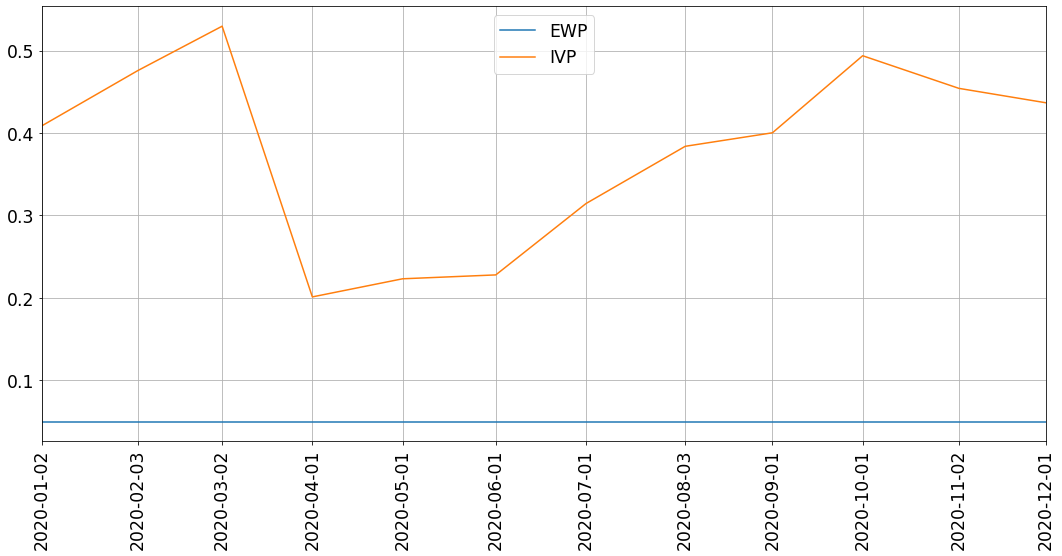
\includegraphics[width=1.15\textwidth]{bilder/nHHI_EWP_and_IVP.png}
            \caption{nHHI over Time}
            \label{fig:nHHI_EWP_and_IVP}
        \end{figure}
        
        Table \ref{tab:ewp_ivp_sharpe_turnover} presents the risk-adjusted returns and turnover of both naive strategies. Inverse variance portfolios achieve a Sharpe ratio almost three times higher than the Sharpe ratio of the equal weight portfolio. The turnover of the IVP is also higher than the turnover of the EWP by a factor of 2.
        
        % Data
        \begin{table}[h]
            \centering
            \begin{tabular}{crr}
             \textbf{Portfolio Optimisation Method} & \textbf{Sharpe Ratio} & \textbf{Turnover} \\
             \hline
             EWP & 0.36 & 0.003634 \\
             IVP & 1.008 & 0.007396
            \end{tabular}
            \caption{Sharpe Ratio and Turnover Figures}
            \label{tab:ewp_ivp_sharpe_turnover}
        \end{table}
        
    \subsection{Practical Implementation of Markowitz's Minimum Volatility Portfolios}\label{section:MarkowitzPracticalImplementation}
        %\textit{In this section, I will describe the optimal portfolios computed within the practical implementation framework}
        
        Now, we continue with the results of the implementation of Markowitz's minimum volatility portfolios from definition \ref{definition:MinimumVolatilityPortfolio}. But first, we describe how the algorithm \ref{algorithm:MMVP} was implemented in detail.
    	
    	For the practical implementation, we use SciPy's linear system solver which can take certain structural properties of the quadratic matrix that defines the linear system, and uses that information to select the method with which to solve the linear system. We take advantage of the fact that the sample covariance matrix is always symmetric and positive-semidefinite. In case the sample covariance matrix has full rank, then it is even positive-definte. Hence, we first assume the sample covariance matrix to be positive-definite, and use this structural property as input for the \texttt{scipy.linalg.solve} method. As a result, the solver will try to solve the linear equation system in definition \ref{definition:MinimumVolatilityPortfolio} using the \textit{LAPACK ?POSV linear equation routine} \cite{scipylinalgsolve}, which tries to solve linear equation systems using the Cholesky decomposition \cite{lapackposv}. In case the method fails to compute a solution to the linear system, then we know that the sample covariance matrix does not have full rank, in which case the practical implementation turns to \texttt{numpy.linalg.lstsq}, which is a NumPy method to compute the least-squares solution to a linear matrix equation \cite{lstsqnumpy}. However, all the covariance matrices computed during the backtesting period have full rank, and the least-squares solver was not used to compute any of the minimum variance portfolios presented here.
    	
    	\begin{theorem}[Cholesky Decomposition]\todo[inline]{Citing Liesens lecture notes ok?}
    		Let $A \in \mathbb{C}^{N \times N}$ be a symmetric positive-definite matrix, then there exists a uniquely determined lower triangular matrix $L \in \mathbb{C}^{N \times N}$ with positive diagonal elements, such that
    		\begin{align}
    			A = L L^H.
    		\end{align}
    	\end{theorem}
    	
    	Figure \ref{fig:MMVP_allocation_plot} shows the evolution of allocations in Markowitz minimum volatility portfolios over time. The changes in allocation are clearly more pronounced than in the case of IVPs (see figure \ref{fig:ivp_allocation_plot}), specially around the start of the COVID-19 (March 2020) crisis when correlations as well as the variance of returns rose and all asset classes suffered negative returns.
        
        % Data
        \begin{figure}[h]
            \centering
            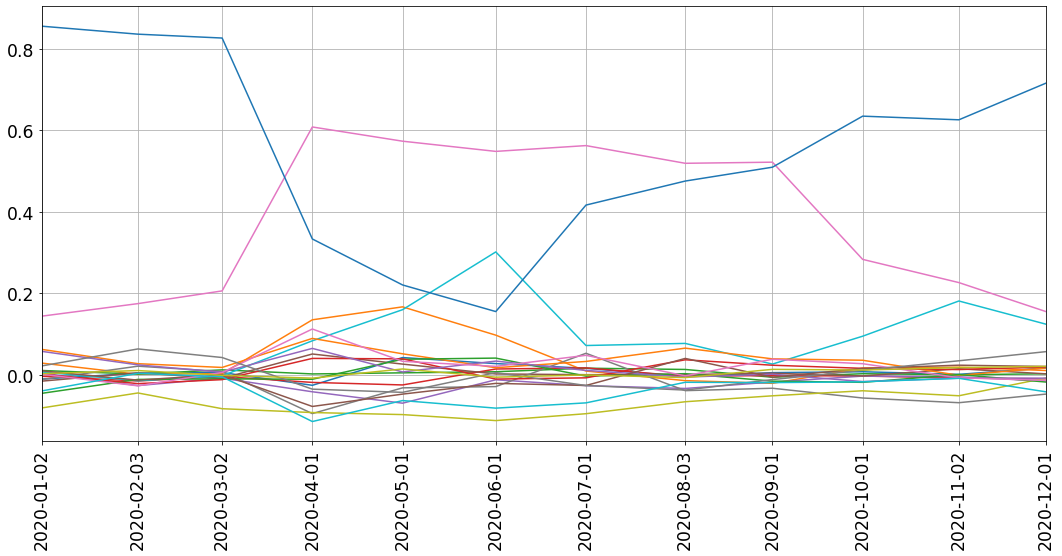
\includegraphics[width=1.15\textwidth]{bilder/MMVP_allocation_plot.png}
            \caption{MMVP Target Allocation over Time}
            \label{fig:MMVP_allocation_plot}
        \end{figure}
        
        The concentration of MMVPs measured by the nHHI remains however lower than in IVPs over the whole backtesting period as figure \ref{fig:nHHI_EWP_IVP_MMVP} shows. Nevertheless, a drop in concentration can be observed following the start of the COVID-19 crisis.
        
        % Data
        \begin{figure}[h]
            \centering
            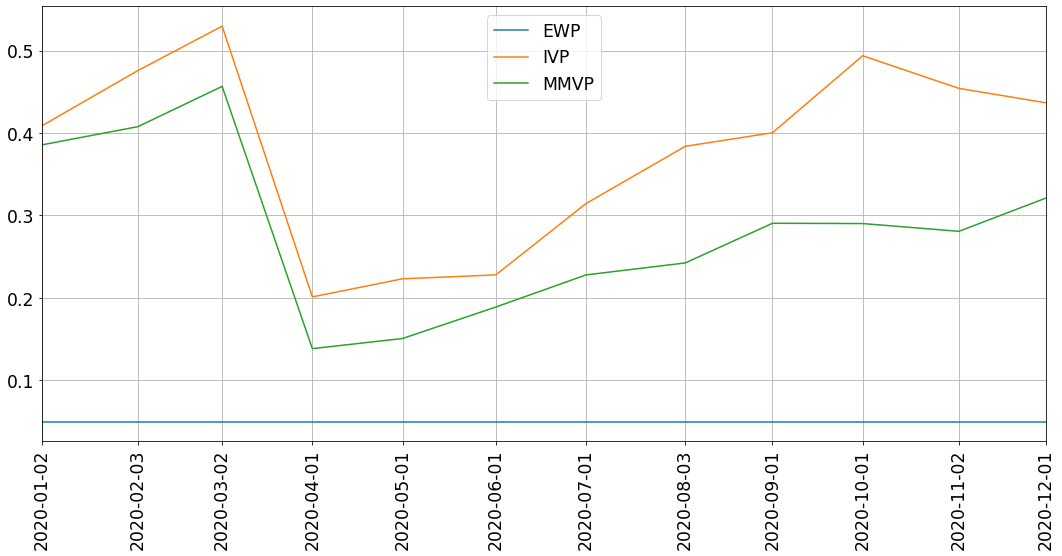
\includegraphics[width=1.15\textwidth]{bilder/nHHI_EWP_IVP_MMVP.png}
            \caption{nHHIn over Time}
            \label{fig:nHHI_EWP_IVP_MMVP}
        \end{figure}
        
        With respect to risk-adjusted returns, MMVPs deliver significantly worse results than both naive allocation methods. The Sharpe ratio of Markowitz's strategy is even negative, i.e. MMVPs fail to generate positive returns during the backtesting period. Moreover, the turnover is also significantly higher than in the case of both naive portfolio optimisation models, as seen in table \ref{tab:ewp_ivp_mmvp_sharpe_turnover}.
        
        % Data
        \begin{table}[h!]
            \centering
            \begin{tabular}{crr}
             \textbf{Portfolio Optimisation Method} & \textbf{Sharpe Ratio} & \textbf{Turnover} \\
             \hline
             EWP & 0.36 & 0.003634 \\
             IVP & 1.008 & 0.007396 \\
             MMVP & -0.017 & 0.018856
            \end{tabular}
            \caption{Sharpe Ratio and Turnover Figures}
            \label{tab:ewp_ivp_mmvp_sharpe_turnover}
        \end{table}
        
        \subsubsection{Markowitz's Curse}\label{section:MarkowitzsCurse}
            %\textit{Using the results of the practical implementation, the concept of Markowitz's is defined here. Moreover, I will provide some mathematical explanation by computing the condition number of the covariance matrices used in the practical implementation and relating them to the error bounds we saw in Numerical Linear Algebra I}
            \todo[inline]{Liesen: Grundsätzliche Frage: Geht es hier um Matrizen, die möglichst nah an I sein sollen oder um gut konditionierte Matrizen? Das sollte noch besser herausgearbeitet werden.}
            
            %References: \cite{lopezmain}
    		
    		To picture the source of instability in the optimisation problem presented in definition \ref{definition:MinimumVolatilityPortfolio}, we can define a forward error bound for its solution based on the condition number of the matrix that defines it, i.e. the sample covariance matrix.
    		
    		\begin{definition}[Condition Number of a Matrix]\todo[inline]{Citing Liesens lecture notes ok?}
    		    If $A \in \mathbb{C}^{N \times N}$ is non-singular, and $\| \cdot \|$ is a norm on $\mathbb{C}^{N \times N}$, then
    		    \begin{align*}
    		        \kappa(A) := \| A \| \| A^{-1} \|
    		    \end{align*}
    		    is called the \textbf{condition number of $A$ with respect to the norm $\| \cdot \|$}.
    		\end{definition}
    		
    		For the results presented here, we compute the condition number with respect to the spectral norm, i.e. with respect to the matrix norm induced by the Euclidean vector norm.
    		
    		\begin{theorem}[Residual-based forward Error Bound]\todo[inline]{Citing Liesens lecture notes ok?}
    			Let $A \in \mathbb{C}^{N \times N}$ be non-singular, $x \in \mathbb{C}^N \setminus \{ 0 \}$ and $b = Ax$. Then for every $\Tilde{x} \in \mathbb{C}^N$ we have
    			\begin{align*}
    				\frac{\| \Tilde{x} - x \|_2}{\| x \|_2} \leq \kappa(A) \frac{\| r \|_2}{\| b \|_2},
    			\end{align*}
    			where $r := b - A \Tilde{x}$ is the residual and $\| r \| / \| b \|$ is the relative residual norm.
    		\end{theorem}
    		
    		\begin{proof}
    			Using $x = A^{-1} b$ and the definition of the residual get
    			\begin{align*}
    				\| \Tilde{x} - x \|_2 = \| A^{-1} (A \Tilde{x} - b)\|_2 \leq \| A^{-1} \| \| r \|_2 = \kappa(A) \frac{\| r \|_2}{\| A \|_2}.
    			\end{align*}
    			
    			Moreover, $\| b \|_2 \leq \| A \|_2 \| x \|_2$ gives
    			\begin{align*}
    				\frac{1}{\| x \|_2} \leq \frac{\| A \|_2}{\| b \|_2},
    			\end{align*}
    			which implies the desired inequality.
    		\end{proof}
    		
    		As we can see, the forward error of the solution computed depends, not only on the relative residual norm, but also on the condition number of the matrix that defines the linear system, in our case the sample covariance matrix. That means, that even if the relative residual norm of the solution is "very small", i.e. the computed solution appears to be very near to the actual solution, a "large" sample covariance matrix condition number implies that the computed solution might actually be very different to the actual solution.\footnote{The terms "very small" and "large" are, obviously, no mathematical terms. A mathematical definition depends on the problem set-up and the error tolerance that can be assumed according to the practical use of the solution. Here, we would like to focus on how changes in the condition number lead to portfolio instability, rather than on how a high or low condition number in absolute terms affects the use of the computed solution.}
    		
    		\begin{theorem}\label{theorem:ConditionNumberEigenvalue}
    		    Let $A \in \mathbb{C}^{N \times N}$ be a non-singular symmetric matrix and $\lambda_1, \dots, \lambda_N$ its eigenvalues, then the condition number of $A$ with respect to the spectral norm is given by \todo[inline]{Liesen: Add source?}
    		    \begin{align*}
    		        \kappa_2(A) := \frac{\max_{i = \{1, \dots, N \} } | \lambda_i |}{\min_{i = \{1, \dots, N \} } | \lambda_i |}.
    		    \end{align*}
    		\end{theorem}
    		
    		\begin{proof}
    		    If $A \in \mathbb{C}^{N \times N}$ is a non-singular symmetric matrix, then we know that $A$ can be unitarily diagonalised:
    		    \begin{align*}
    		        A = U \Lambda U^H,
    		    \end{align*}
    		    where $U \in \mathbb{C}^{N \times N}$ is an unitary matrix and $\Lambda := diag(\lambda_1, \dots, \lambda_N) \in \mathbb{C}^{N \times N}$ is a diagonal matrix that contains the eigenvalues of $A$ in the diagonal. Using the fact that the spectral norm is unitarily invariant, we get
    		    \begin{align*}
    		        \kappa_2(A) &= \| A \|_2 \| A^{-1} \|_2 \\
    		        &= \| U \Lambda U^H \|_2 \| (U \Lambda U^H)^{-1} \|_2 \\
    		        &= \| \Lambda \|_2 \| \Lambda^{-1} \|_2 \\
    		        &= \max_{i = \{1, \dots, N \} } | \lambda_i | \frac{1}{\min_{i = \{1, \dots, N \} } | \lambda_i |} = \frac{\max_{i = \{1, \dots, N \} } | \lambda_i |}{\min_{i = \{1, \dots, N \} } | \lambda_i |}.
    		    \end{align*}
    		\end{proof}
    		
    		Using the decomposition of the covariance matrix from definition \ref{definition:CovarianceMatrix}
    		\begin{align*}
    		    \Sigma = S P S,
    		\end{align*}
    		where $S$ is the standard deviation matrix and $P$ the correlation matrix, and the result of theorem \ref{theorem:ConditionNumberEigenvalue}, we see that condition number of the covariance matrix is minimal for a fixed standard deviation matrix when the correlation matrix is a diagonal matrix, and for a fixed correlation matrix when the standard deviation of all assets' returns is equal. The first case follows from the fact that the diagonal entries of the correlation matrix are always equal to $1$, because all assets are perfectly correlated to themselves. A diagonal correlation matrix corresponds to a set of assets that are uncorrelated. As the relative difference in the standard deviation of the assets and their correlations rise, the condition number of the corresponding sample covariance matrix also rises. This tends to happen during periods of market stress, when investors fear the fall of asset prices across asset classes, sectors and countries. However, it is exactly during those periods of market stress when investors do need to make the most out of diversification to reduce the impact of price fall in their aggregated portfolio. This issue is what López de Prado calls \textit{Markowitz's curse} \cite{lopezmain}:
    		
    		\begin{displayquote}
    		    "The more correlated the investments, the greater the need for diversification, and yet the more likely we will receive unstable solutions. The benefits of diversification often are more than offset by estimation errors."
            \end{displayquote}
            
            Moreover, periods of market stress tend to start suddenly, and investors reactions are drastic, which in turn causes sudden sharp rises in the condition number of the covariance matrix. As a result, the covariance matrices used to compute the optimal portfolios at the last and first rebalancing point just before and just after the period of market stress respectively tend to be very different, potentially generating very different optimal allocations. This is one of the reasons why Markowitz's minimum volatility portfolios tend to be more unstable across time, generating higher transaction costs.
    		
    		In figure \ref{fig:LopezdePrado_Corr_Eig_Plot}, we can see the eigenvalues of different types of correlation matrices plotted from López de Prado's paper \cite{lopezmain}, in this case correlations matrices of size $50$. The ideal correlation matrix is the identity matrix, which has $\lambda = 1$ as unique eigenvalue and hence condition number equal to $1$. As we add correlated assets to our universe, the largest eigenvalue in modulo of the correlation matrix increases while the smallest eigenvalue in modulo decreases leading to an increase of its condition number.
    		
    		\begin{figure}[h!]
    			\centering
    			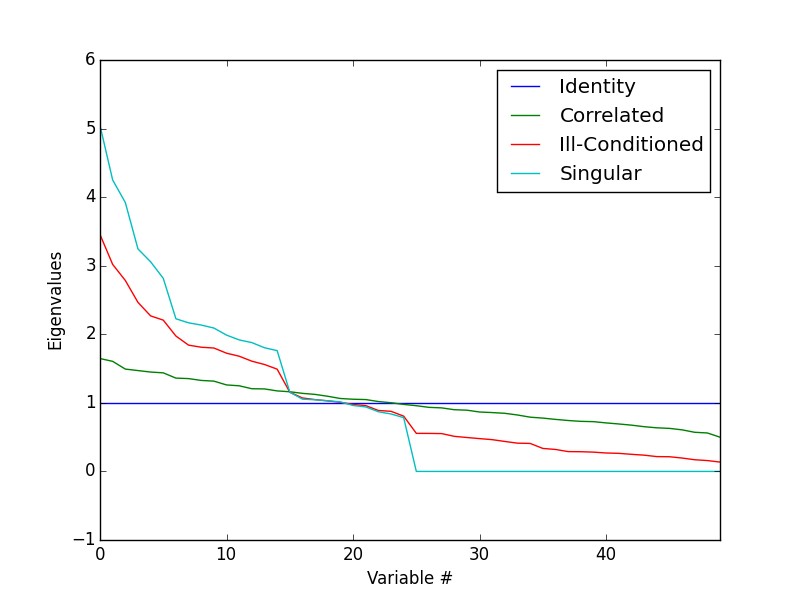
\includegraphics[width=1.15\textwidth]{bilder/LopezdePrado_Corr_Eig_Plot.png}
    			\caption{Visualisation of Markowitz's Curse \cite{lopezmain}}
    			\label{fig:LopezdePrado_Corr_Eig_Plot}
    		\end{figure}
    		
    		To quantify how correlated assets are, we define the following distance measure for the distance between each of the computed correlation matrices corresponding to each sample covariance matrix of our practical implementation and the \textit{ideal} correlation matrix\footnote{We consider the identity matrix as the ideal correlation matrix because it maximises the stability of the optimisation method. Furthermore, of all possible correlation matrices, a set of perfectly uncorrelated assets used as input for Markowitz's portfolio optimisation method results in the portfolio with the lowest variance. For other purposes, a correlation matrix equal to the identity matrix might not be ideal.}, i.e. the identity matrix.
    		
    		\begin{definition}
    		    Let $\Omega \in \mathbb{R}^{N \times N}$ be a correlation matrix as in definition \ref{definition:CovarianceMatrix}. We define the \textbf{distance of $\Omega$ to the ideal correlation matrix} as
    		    \begin{align*}
    		        \| \Omega - I_N \|_F,
    		    \end{align*}
    		    where $\| \cdot \|_F$ is the Frobenius norm and $I_N$ is the $N$-dimensional identity matrix. Obviously,
    		    \begin{align*}
    		        \| \Omega - I_N \|_F \geq 0
    		    \end{align*}
    		    holds for all correlation matrices $\Omega \in \mathbb{R}^{N \times N}$.
    		\end{definition}
    		
    		The distance of a correlation matrix to the ideal correlation matrix that we have just defined is a measure of how much different assets are correlated (positively as well as negatively). The more correlated assets are, the higher the distance to the ideal correlation matrix, which corresponds to all assets being completely uncorrelated.
    		
    		Figure \ref{fig:Corr_dist_to_id} shows the change in the distance of the correlation matrices corresponding to the computed covariance matrices over the backtesting period. We can appreciate a steep rise in the distance coinciding with the start of the COVID-19 crisis, showing how strong the correlations between the assets in our universe rose. Correlations remained high until October, and later failed to get back down to the levels observed at the beginning of the backtesting period. In this figure, we can also observe that the rises can be very sudden and steep.
    		
    		\begin{figure}[h!]
    		    \centering
    		    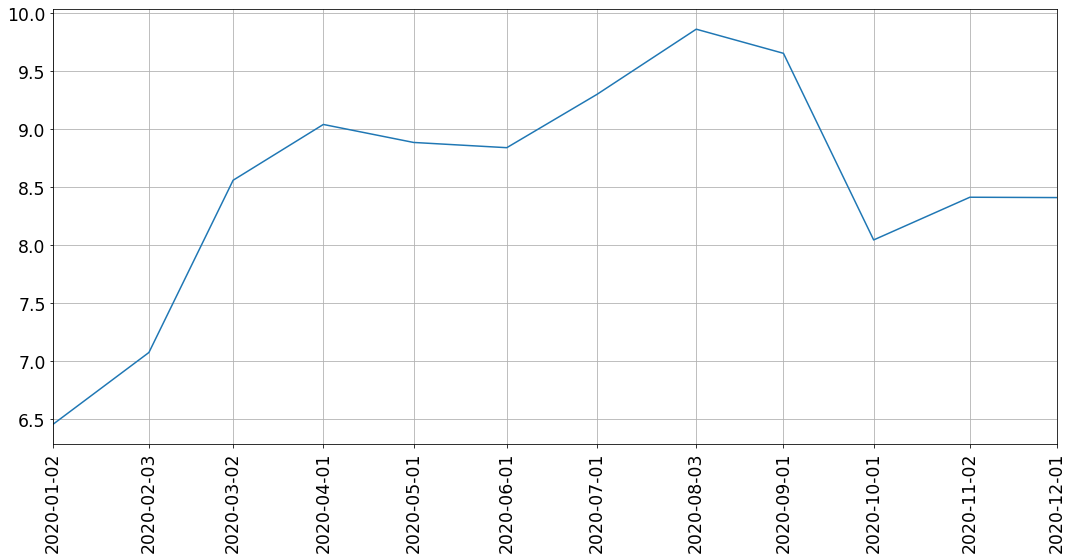
\includegraphics[width=1.15\textwidth]{bilder/Corr_dist_to_id.png}
    		    \caption{Correlation Matrix Distance to Ideal Correlation Matrix over the Backtesting Period}
    		    \label{fig:Corr_dist_to_id}
    		\end{figure}
    		
    		We quantify the condition number with respect to the spectral norm of the covariance matrices used for the computation of Markowitz minimum volatility portfolios in our practical implementation, as well as the ones of the correlation and variance matrices corresponding to those covariance matrices. The results are plotted in figure \ref{fig:Cov_corr_var_matrix_cond}. A clear sudden sharp rise in the condition number of the sample covariance matrix can be observed at the beginning of the COVID-19 crisis, when lock-downs and other measures that slowed down economies worldwide were enacted. This rise in the condition number of the sample covariance matrix was initially driven by a steep rise in correlations, as the condition number of the correlation matrix and figure \ref{fig:Corr_dist_to_id} show. However, as the variances of returns across the assets in our portfolio universe rose, they also got to similar levels, which in turn led to a sharp drop in the condition number of the variance, and hence also of the covariance, matrix. Economically speaking, as the COVID-19 crisis started, investors initially decided to liquidate their holdings across all assets classes, and increase their cash allocation. This led to a reduction in the relatively wide difference in returns' variance between more conservative asset classes, like fixed-income, and more aggressive asset classes, like equities and commodities, that prevails during normal times. In second half of the year, correlations remained high, and variances returned to more normal levels, leading to a new increase in the condition number of the sample covariance matrix to even higher levels than in the first half of the year, as the advantageous effects of higher, more similar variances across the assets disappeared.
    		
    		\begin{figure}[h!]
    		    \centering
    		    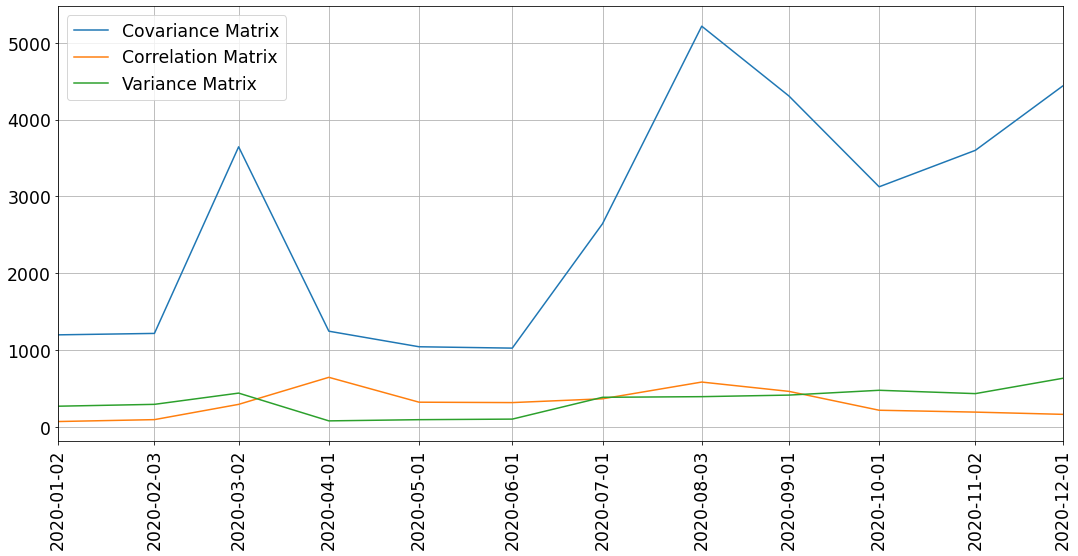
\includegraphics[width=1.15\textwidth]{bilder/Cov_corr_var_matrix_cond.png}
    		    \caption{Condition Number of the Covariance and its Corresponding Correlation and Variance Matrices over the Backtesting Period}
    		    \label{fig:Cov_corr_var_matrix_cond}
    		\end{figure}
    		
    		The effects of the changes in the condition number of the sample covariance matrix can be observed in figure \ref{fig:nHHI_EWP_IVP_MMVP}, where the changes in concentration track the changes in the condition number of the sample covariance matrix, and in figure \ref{fig:Turnover_over_time_EWP_IVP_MMVP}, where the turnover of the MMVP is almost twice as high as the turnover of the IVP\footnote{The inverse variance portfolio (IVP) is actually Markowitz's minimum volatility portfolio (MMVP) computed using the ideal correlation matrix. See remark \ref{remark:IVPEquivalentToMMVP}.}.
    		
    		\begin{figure}[h!]
    		    \centering
    		    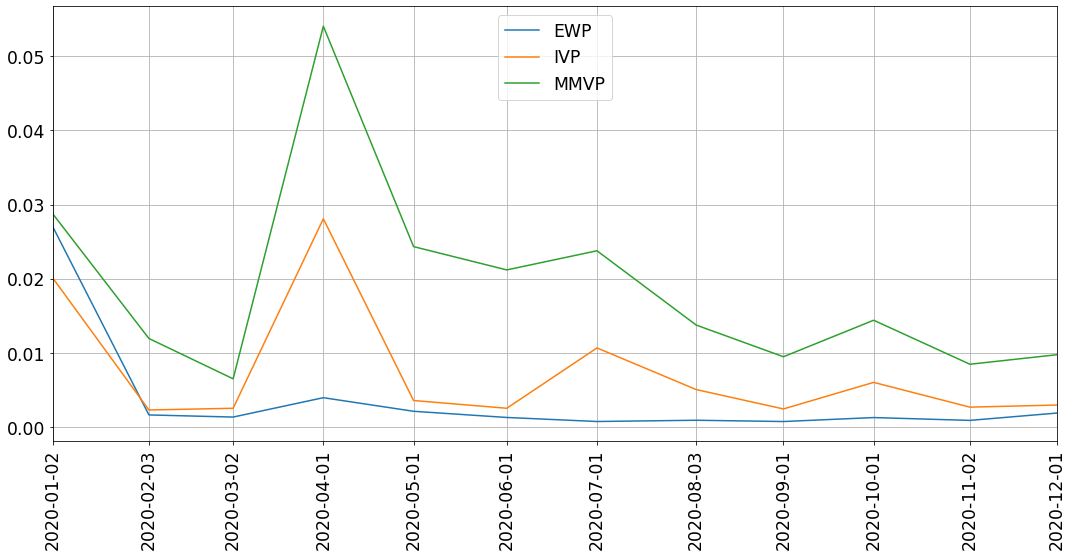
\includegraphics[width=1.15\textwidth]{bilder/Turnover_over_time_EWP_IVP_MMVP.png}
    		    \caption{Turnover of EWP, IVP and MMVP over the Backtesting Period}
    		    \label{fig:Turnover_over_time_EWP_IVP_MMVP}
    		\end{figure}
    	
    	We conclude that even if the condition number of the covariance matrices used for the computation of Markowitz's minimum volatility portfolios in our practical implementation is relatively low to produce high residual-based forward error bounds, the stability of the portfolio allocation over time suffered from sudden sharp rises in correlations between assets, as well as from sudden sharp changes in the relative difference between the variance of returns of rather "safe" assets like fixed-income ETFs and "riskier" assets like equity ETFs. Another interesting finding is the fact that the stronger rise in returns' variance of "safer" assets, which exhibit lower variances in normal times, than that of "riskier" assets had a cushion effect, sinking the condition number of the covariance matrix at the start of the COVID-19 crisis and reducing portfolio turnover in the last half of the year. Finally, Markowitz's minimum volatility portfolios fail to perform better than the two naive portfolio allocation models defined above, producing higher portfolio turnover and even negative risk-adjusted returns.